\subsubsection{Mechanischer Aufbau}
\chapterauthor{Philipp Thaler}
%Philipp, Matthias und Lukas

In diesem Abschnitt wird auf den mechanischen Aufbau des Systems eingegangen.

\begin{figure}[htpb] % {H}
    \centering
    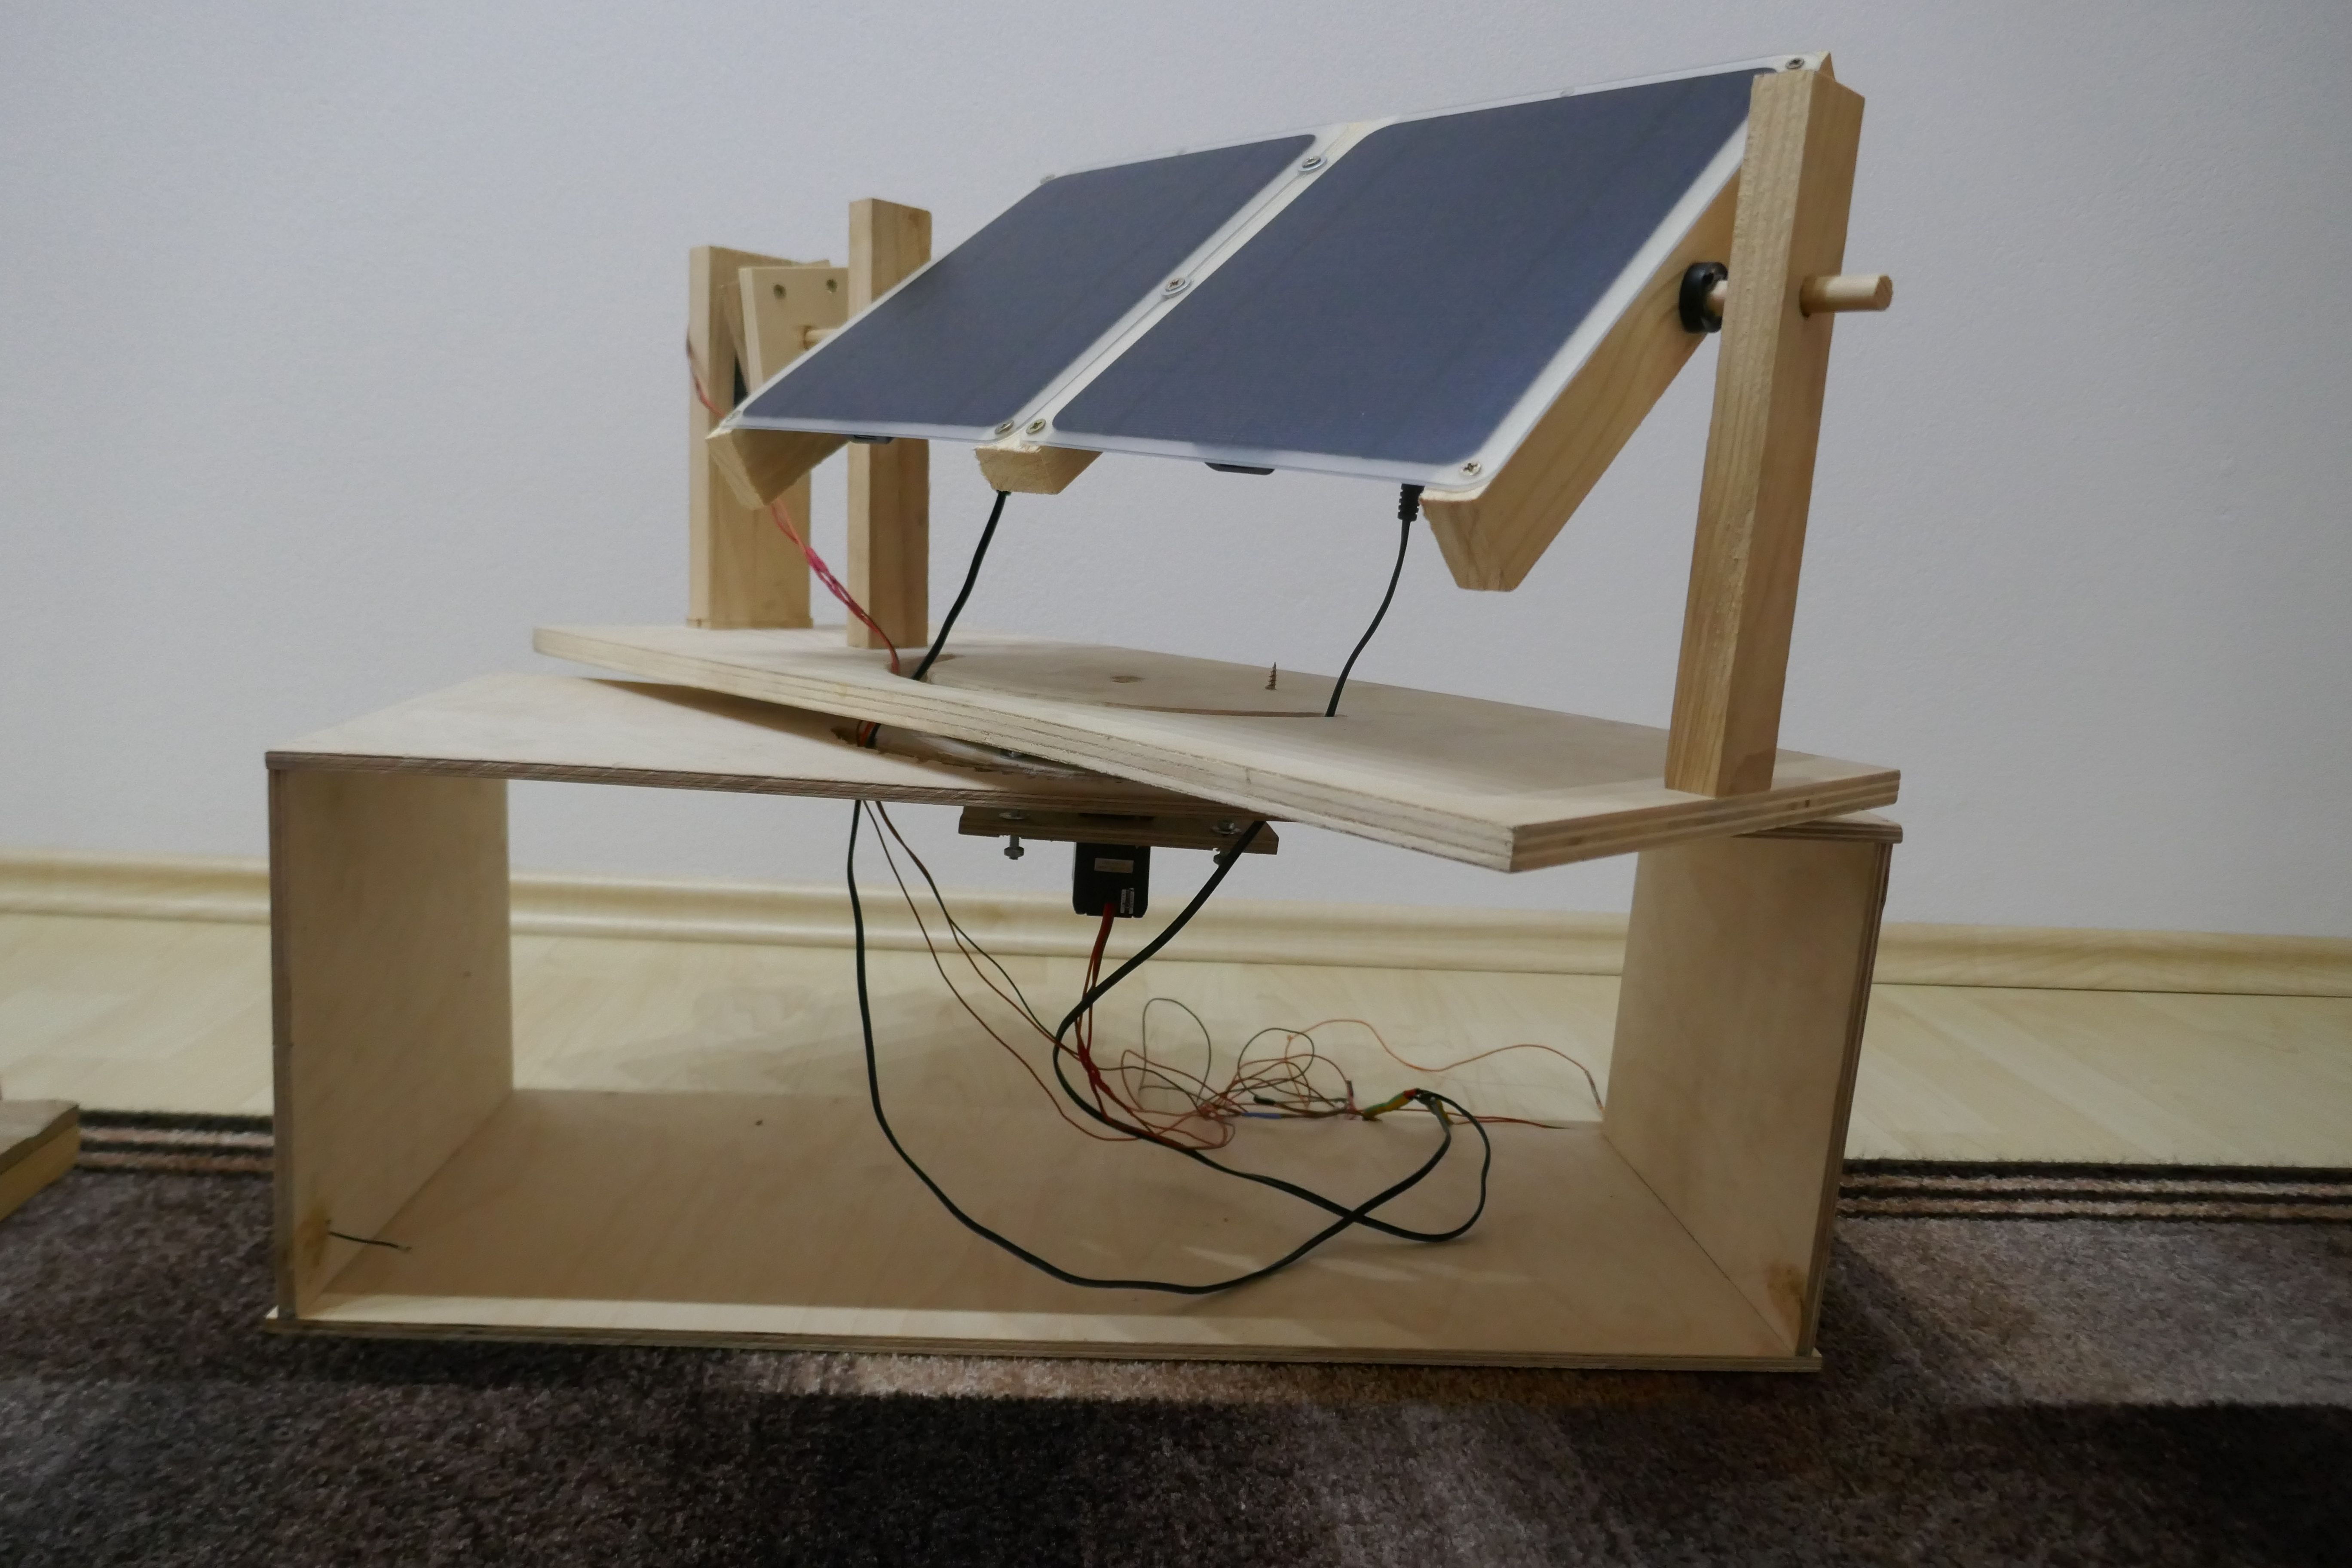
\includegraphics[width=13cm,keepaspectratio=true]{pics/aufbau_seitenansicht.JPG}
    \caption{Aufbau des Systems}\label{aufbauSeitenansicht}
\end{figure}

\autoref{aufbauSeitenansicht} zeigt die Holzkonstruktion mit den beiden Servomotoren und den Solarmodulen.

Die beiden Solarplatten sind auf Holzlatten festgeschraubt. 
Um eine Drehung von 180° zu ermöglichen, sind die Holzlatten auf einem Holzstab befestigt.
Dieser wird von den beiden Stützhölzern links und rechts gehalten. 
Der Servomotor, der für die Neigung der Solarmodule verantwortlich ist, sitzt auf einer eigenen Stütze, wie im Hintergrund von \autoref{aufbauLagerung} zu erkennen.

Eine Schwierigkeit ist, den Servomotor mit der Stange auf dem die Module gelagert sind, zu verbinden.
Hierzu wird der Hebel des Servomotors an ein Holzquadrat geschraubt, welches ebenso an dem Holzstab befestigt ist.
Vor dem Anbringen muss der Motor in eine der beiden Nullstellungen gebracht werden.
Die Solarmodule werden um 90° zur Bodenplatte geneigt, um eine Nullstellung als Ausgangspunkt zu erhalten. 
Somit ist es dem oberen Servomotor möglich, die Solarmodule um 90° in beide Richtungen zu neigen.

\begin{figure}[htpb] % {H}
    \centering
    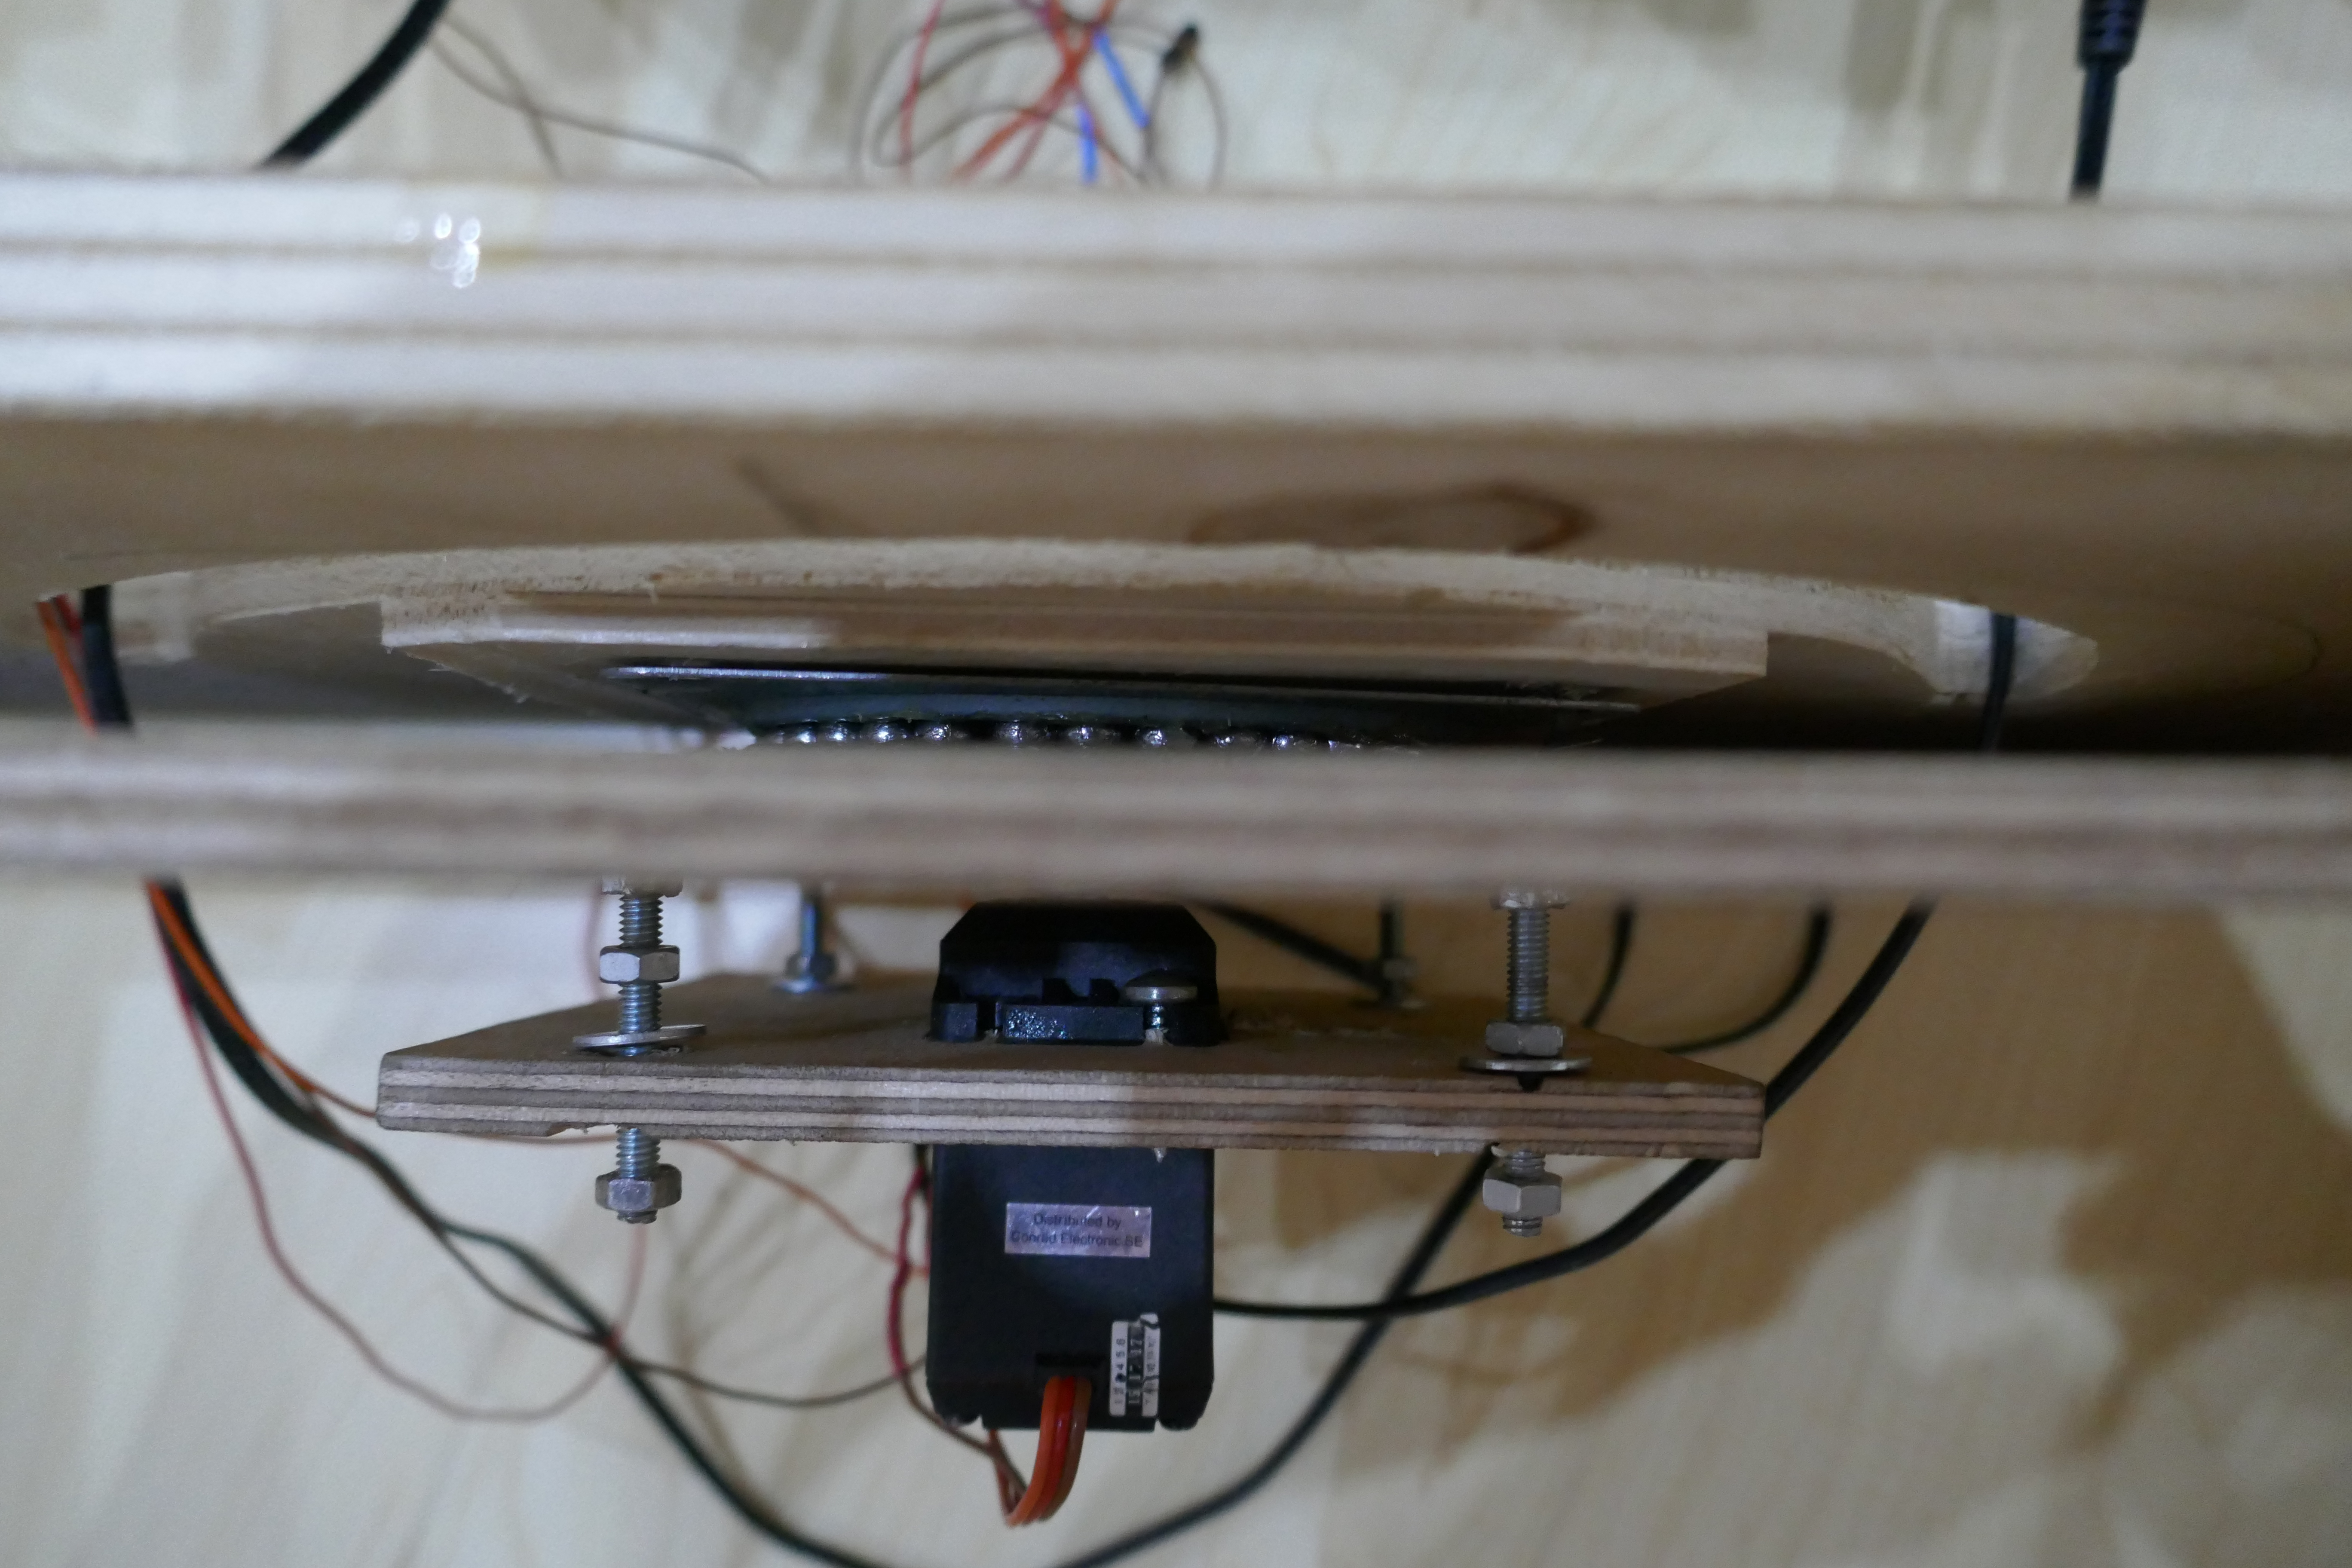
\includegraphics[width=13cm,keepaspectratio=true]{pics/aufbauLagerung.JPG}
    \caption{Lagerung der oberen Konstruktion}\label{aufbauLagerung}
\end{figure}

\autoref{aufbauLagerung} zeigt, wie die obere Konstruktion mit der unteren Holzkonstruktion verbunden ist.
In der Mitte ist das verwendete Kugellager zu erkennen. 
Dieses ist durch vier Schrauben mit der oberen Platte verbunden und ermöglicht dem unteren Servomotor den gesamten Oberbau um 180° zu drehen.

Hierbei ist die Schwierigkeit den unteren Servomotor mit der oberen Platte zu verbinden. 
Dazu wird in die obere Platte der Unterkonstruktion ein Loch in der Mitte ausgeschnitten, um den Servohebel an die Bodenplatte der Oberkonstruktion anzubringen.
Nun kann der untere Servomotor mit den vier langen Schrauben und einem Holzeinsatz unten an den Servohebel gepresst werden. 
Um nicht zu viel Druck auf den Servomotor auszuüben, sind Gegenmuttern angebracht.

In \autoref{aufbauLagerung} ist zu erkennen, wie die Kabeldurchführung der Solarmodule und des oberen Servomotors gehandhabt wird. 
Hierzu wird ein etwa 1 cm dicker Halbkreisbogen ausgeschnitten. 
Somit können sich die Kabel auch bei der Rotation der Basis frei bewegen und behindern die Rotation nicht.